\documentclass[12pt, letterpaper]{article}

% ── Packages ──────────────────────────────────────────────
\usepackage[margin=1in]{geometry}
\usepackage{amsmath, amssymb, amsthm}
\usepackage{graphicx}
\usepackage{booktabs}
\usepackage{longtable}
\usepackage{hyperref}
\usepackage{listings}
\usepackage{xcolor}
\usepackage{tikz}
\usetikzlibrary{shapes, arrows.meta, positioning, fit, calc}
\usepackage{pgfplots}
\pgfplotsset{compat=1.18}
\usepackage{float}
\usepackage{caption}
\usepackage{subcaption}
\usepackage{algorithm}
\usepackage{algpseudocode}
\usepackage{enumitem}
\usepackage{natbib}
\usepackage{tcolorbox}
\usepackage{fancyhdr}

% ── Page Style ────────────────────────────────────────────
\pagestyle{fancy}
\fancyhf{}
\rhead{Tavares \& White}
\lhead{Polymarket Pricing Gap Detection}
\cfoot{\thepage}

% ── Code Listing Style ───────────────────────────────────
\definecolor{codegreen}{rgb}{0,0.6,0}
\definecolor{codegray}{rgb}{0.5,0.5,0.5}
\definecolor{codepurple}{rgb}{0.58,0,0.82}
\definecolor{backcolour}{rgb}{0.95,0.95,0.95}
\lstdefinestyle{mystyle}{
    backgroundcolor=\color{backcolour},
    commentstyle=\color{codegreen},
    keywordstyle=\color{codepurple},
    numberstyle=\tiny\color{codegray},
    stringstyle=\color{codegreen},
    basicstyle=\ttfamily\footnotesize,
    breakatwhitespace=false,
    breaklines=true,
    captionpos=b,
    keepspaces=true,
    numbers=left,
    numbersep=5pt,
    showspaces=false,
    showstringspaces=false,
    showtabs=false,
    tabsize=2,
    frame=single
}
\lstset{style=mystyle}

% ── Title ─────────────────────────────────────────────────
\title{%
  \textbf{Multi-Agent Pricing Gap Detection in Decentralized Prediction Markets:}\\[6pt]
  \large A Big Data Architecture for Sentiment-Driven Inefficiency Discovery on Polymarket
}
\author{
  Nicholas Tavares\thanks{Stevens Institute of Technology, MS Applied Mathematics} \quad
  Matthew White\thanks{Stevens Institute of Technology}
}
\date{March 2026}

\begin{document}
\maketitle

% ══════════════════════════════════════════════════════════
% ABSTRACT
% ══════════════════════════════════════════════════════════
\begin{abstract}
Prediction markets aggregate dispersed information into asset prices through continuous trading, theoretically achieving informational efficiency. This paper presents a multi-agent system built on CrewAI, PostgreSQL, and large language model (LLM) ensemble sentiment analysis to detect pricing gaps in Polymarket---the largest decentralized prediction market by volume. Our system integrates eight heterogeneous data sources (Polymarket Gamma API, Bluesky AT Protocol, GDELT, RSS aggregation, Reddit mirror scraping, X/Nitter mirror scraping, Tavily web search, and cross-market APIs), processes over 32,000 social posts across 625 tracked contracts, and applies a four-type gap detection framework: sentiment-probability mismatches, information asymmetry, historical pattern deviations, and cross-market arbitrage. After four complete analytical cycles spanning March 19--21, 2026, the system detected 30 pricing gaps---29 sentiment mismatches and 1 cross-platform arbitrage---none of which have been validated against market resolution. Analysis of the detected gaps reveals systematic social media optimism bias rather than genuine market inefficiency, with fan-driven sentiment on sports contracts constituting the majority of false positives. We present evidence consistent with weak-form market efficiency in liquid Polymarket contracts and discuss the fundamental speed disadvantage of daily-frequency sentiment analysis against markets that incorporate information on the order of minutes. We conclude with a discussion of prediction market odds as potential input features for equity forecasting models, representing a more viable application of this infrastructure.

\medskip
\noindent\textbf{Keywords:} prediction markets, market efficiency, multi-agent systems, sentiment analysis, big data, NLP, CrewAI, Polymarket, pricing gaps, information aggregation
\end{abstract}

\newpage
\tableofcontents
\newpage

% ══════════════════════════════════════════════════════════
\section{Introduction}
% ══════════════════════════════════════════════════════════

\subsection{Motivation}

Prediction markets---platforms where participants trade contracts on the outcomes of future events---have emerged as powerful mechanisms for information aggregation \citep{arrow2008promise}. Unlike traditional polling or expert forecasting, prediction markets incentivize truthful revelation of beliefs through financial stakes, theoretically producing prices that reflect the collective wisdom of informed participants \citep{wolfers2004prediction}.

Polymarket, launched in 2020 on the Polygon blockchain, has become the dominant decentralized prediction market, processing over \$1 billion in trading volume during the 2024 U.S. presidential election cycle alone. Its transparent order book, low transaction costs, and broad market coverage create an environment where the Efficient Market Hypothesis (EMH) can be empirically tested in a novel asset class.

The central question of this research is: \textbf{Can a multi-agent AI system, leveraging heterogeneous social media sentiment and cross-platform data fusion, systematically identify pricing inefficiencies in prediction markets before they are corrected by market participants?}

\subsection{Theoretical Framework}

Our work sits at the intersection of three bodies of literature:

\begin{enumerate}[label=(\roman*)]
    \item \textbf{Market Microstructure Theory.} Kyle's (1985) model of informed trading establishes that market efficiency is a function of the rate $\lambda$ at which market makers learn from order flow. In prediction markets with transparent order books, $\lambda$ approaches instantaneous for liquid contracts, implying that information asymmetries are resolved rapidly \citep{kyle1985continuous}.

    \item \textbf{Prediction Market Efficiency.} Manski (2006) demonstrates that prediction market prices can be interpreted as mean beliefs under specific conditions, while Rothschild (2009) shows that prediction markets outperform polls in election forecasting, suggesting genuine information aggregation \citep{manski2006interpreting}.

    \item \textbf{Sentiment Analysis for Financial Prediction.} Bollen et al.\ (2011) demonstrate that Twitter sentiment predicts DJIA movements with 87.6\% accuracy, while more recent work questions whether LLM-derived sentiment adds alpha beyond what informed traders already incorporate \citep{bollen2011twitter}.
\end{enumerate}

\subsection{Research Contributions}

This paper makes the following contributions:

\begin{enumerate}
    \item \textbf{Architecture:} We present a production-grade, multi-agent pipeline for real-time prediction market analysis, integrating eight data sources through a CrewAI-orchestrated four-agent system with PostgreSQL persistence.

    \item \textbf{Empirical Finding:} We provide evidence that detected ``pricing gaps'' in Polymarket are predominantly driven by \textit{social media optimism bias}---a well-documented systematic overweighting of positive sentiment on social platforms---rather than genuine market inefficiency.

    \item \textbf{Big Data Infrastructure:} We demonstrate a scalable architecture processing 32,791 social posts, 12,185 sentiment analyses, and 625 contracts through ensemble NLP (VADER + TextBlob + LLM) with a 9-table PostgreSQL schema, providing a template for large-scale financial text analytics.

    \item \textbf{Negative Result:} We document the failure mode of daily-frequency sentiment analysis against markets with minute-level information incorporation---a cautionary result for researchers and practitioners attempting similar approaches.
\end{enumerate}

% ══════════════════════════════════════════════════════════
\section{System Architecture}
% ══════════════════════════════════════════════════════════

\subsection{Design Philosophy}

The system follows a \textit{sequential multi-agent pipeline} pattern, where each agent specializes in one phase of the analytical workflow. This design was chosen over a monolithic approach for three reasons: (1) modularity enables independent testing and iteration of each component, (2) agent specialization allows LLM prompt engineering to be tailored per task, and (3) CrewAI's process model provides built-in error isolation between phases.

\subsection{Pipeline Architecture}

\begin{figure}[H]
\centering
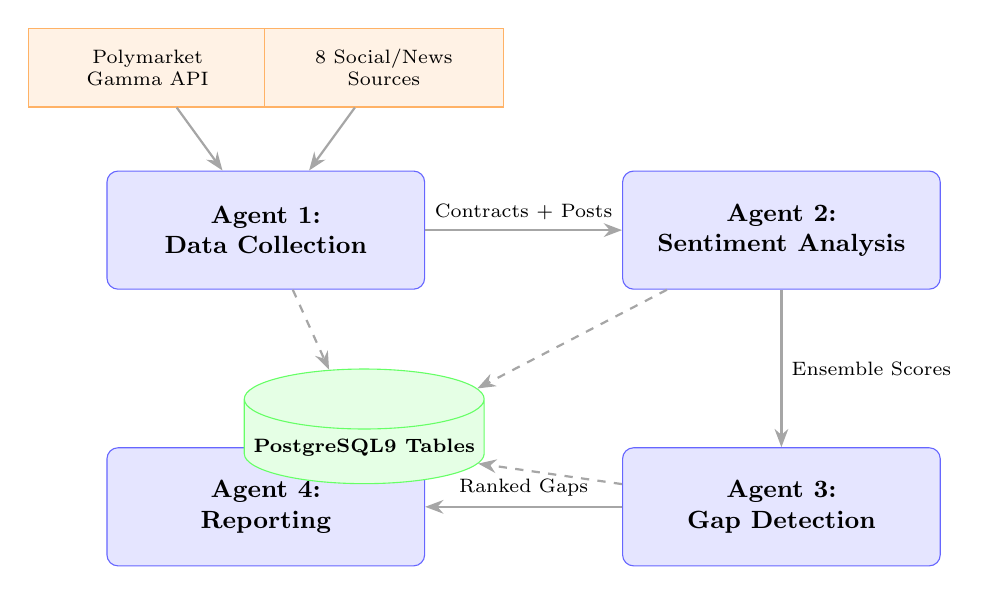
\begin{tikzpicture}[
    node distance=1.8cm,
    agent/.style={rectangle, rounded corners, draw=blue!60, fill=blue!10,
        text width=3.8cm, minimum height=1.5cm, align=center, font=\small\bfseries},
    data/.style={rectangle, draw=orange!60, fill=orange!10,
        text width=2.8cm, minimum height=1cm, align=center, font=\scriptsize},
    db/.style={cylinder, draw=green!60, fill=green!10,
        shape border rotate=90, aspect=0.25, minimum height=1.2cm,
        minimum width=1.8cm, font=\scriptsize\bfseries},
    arrow/.style={-Stealth, thick, draw=gray!70}
]

% Agents
\node[agent] (dc) {Agent 1:\\Data Collection};
\node[agent, right=2.5cm of dc] (sa) {Agent 2:\\Sentiment Analysis};
\node[agent, below=2cm of sa] (gd) {Agent 3:\\Gap Detection};
\node[agent, left=2.5cm of gd] (rp) {Agent 4:\\Reporting};

% Data sources
\node[data, above=0.8cm of dc, xshift=-1.5cm] (poly) {Polymarket\\Gamma API};
\node[data, above=0.8cm of dc, xshift=1.5cm] (social) {8 Social/News\\Sources};

% Database
\node[db, below=1cm of dc, xshift=1.25cm] (pgdb) {PostgreSQL\\9 Tables};

% Arrows
\draw[arrow] (poly) -- (dc);
\draw[arrow] (social) -- (dc);
\draw[arrow] (dc) -- node[above, font=\scriptsize] {Contracts + Posts} (sa);
\draw[arrow] (sa) -- node[right, font=\scriptsize] {Ensemble Scores} (gd);
\draw[arrow] (gd) -- node[above, font=\scriptsize] {Ranked Gaps} (rp);
\draw[arrow, dashed] (dc) -- (pgdb);
\draw[arrow, dashed] (sa) -- (pgdb);
\draw[arrow, dashed] (gd) -- (pgdb);

\end{tikzpicture}
\caption{Four-agent sequential pipeline architecture. Solid arrows indicate data flow; dashed arrows indicate database persistence at each stage.}
\label{fig:architecture}
\end{figure}

The four agents operate sequentially within each cycle:

\begin{enumerate}
    \item \textbf{Data Collection Agent} fetches the full contract universe from the Polymarket Gamma API (paginated, 100 per request), filters and ranks contracts by a composite score (volume 30\%, volatility 25\%, uncertainty 20\%, time pressure 10\%, liquidity 10\%, spread 5\%), and collects social media posts from all enabled sources using a dual-search strategy (keyword extraction + full title search).

    \item \textbf{Sentiment Analysis Agent} processes collected posts in batches of 5 through an ensemble of three models: the primary LLM (DeepSeek, weight = 0.50), VADER lexicon analyzer (weight = 0.25), and TextBlob polarity (weight = 0.25). Results are aggregated into rolling sentiment snapshots at 6-hour, 12-hour, and 24-hour windows.

    \item \textbf{Gap Detection Agent} applies four detection algorithms (detailed in Section~\ref{sec:gap_detection}) to identify pricing discrepancies between market odds and information-implied probabilities.

    \item \textbf{Reporting Agent} ranks detected gaps by a composite score (70\% confidence + 30\% edge percentage) and formats results for console output and CSV export.
\end{enumerate}

\subsection{Technology Stack}

\begin{table}[H]
\centering
\caption{Core technology components and their roles in the system.}
\label{tab:tech_stack}
\begin{tabular}{@{}lll@{}}
\toprule
\textbf{Component} & \textbf{Technology} & \textbf{Role} \\
\midrule
Agent Orchestration & CrewAI 0.28.8 & Sequential multi-agent coordination \\
LLM Integration & LangChain 0.1.20 & LLM abstraction layer \\
Primary LLM & DeepSeek Chat & Sentiment analysis, market matching \\
Fast LLM & Ollama (LLaMA 3.1 8B) & Keyword extraction, lightweight tasks \\
Database & PostgreSQL 12+ & 9-table persistence layer \\
ORM & SQLAlchemy 2.0.30 & Object-relational mapping \\
Web Framework & FastAPI 0.111.0 & Dashboard API (8 endpoints) \\
Sentiment (Lexicon) & VADER 3.3.2, TextBlob 0.18 & Ensemble sentiment components \\
Data Processing & Pandas 2.2.2, NumPy 1.26.4 & Numerical analysis \\
Configuration & Pydantic 2.7.1 & Type-safe settings management \\
Web Scraping & BeautifulSoup4 4.12.3 & Mirror site scraping \\
Rate Limiting & ratelimit 2.2.1 & API throttling \\
\bottomrule
\end{tabular}
\end{table}

\subsection{Data Sources}

The system integrates eight heterogeneous data sources, each accessed through a standardized service interface:

\begin{table}[H]
\centering
\caption{Data source integration summary. Sources marked with $\dagger$ experienced persistent failures during the study period.}
\label{tab:data_sources}
\begin{tabular}{@{}llcll@{}}
\toprule
\textbf{Source} & \textbf{Type} & \textbf{Cost} & \textbf{Protocol} & \textbf{Status} \\
\midrule
Polymarket Gamma API & Market Data & Free & REST & Active \\
Bluesky AT Protocol & Social Media & Free & AT Protocol & Active \\
GDELT & News & Free & REST & Active \\
RSS (Reuters, BBC, AP) & News & Free & feedparser & Active \\
Reddit Mirror (Redlib) & Social Media & Free & Scraping & Active \\
X Mirror (xcancel) & Social Media & Free & Scraping & Active \\
Tavily Web Search$^\dagger$ & Web Search & Paid & REST & Failed (HTTP 432) \\
Grok / xAI$^\dagger$ & Social Media & Paid & REST & Disabled \\
\bottomrule
\end{tabular}
\end{table}

Cross-market data for arbitrage detection is sourced from Kalshi (REST API, free, no authentication) and Manifold Markets (REST API, free).

% ══════════════════════════════════════════════════════════
\section{Database Schema \& Big Data Considerations}
\label{sec:database}
% ══════════════════════════════════════════════════════════

\subsection{Schema Design}

The system persists all data in a PostgreSQL database (\texttt{polymarket\_gaps}) with nine tables designed for both real-time operational queries and historical analysis:

\begin{table}[H]
\centering
\caption{Database schema overview with record counts as of March 21, 2026.}
\label{tab:schema}
\begin{tabular}{@{}llrl@{}}
\toprule
\textbf{Table} & \textbf{Purpose} & \textbf{Records} & \textbf{Key Columns} \\
\midrule
\texttt{contracts} & Full market universe & 625 & question, odds, volume, liquidity \\
\texttt{social\_posts} & Multi-platform posts & 32,791 & platform, content, engagement \\
\texttt{sentiment\_analysis} & Ensemble scores & 12,185 & llm, vader, textblob, ensemble \\
\texttt{detected\_gaps} & Pricing anomalies & 30 & type, confidence, edge, evidence \\
\texttt{historical\_odds} & Price time series & 8 & yes/no odds, volume, timestamp \\
\texttt{sentiment\_snapshots} & Rolling aggregates & varies & 6h/12h/24h windows \\
\texttt{cycle\_runs} & Execution audit & 4 & duration, counts, errors, metadata \\
\texttt{backtest\_results} & Validation metrics & 0 & win\_rate, avg\_edge, ROI \\
\texttt{system\_logs} & Audit trail & varies & level, agent, message \\
\bottomrule
\end{tabular}
\end{table}

\subsection{Big Data Design Patterns}

Several design decisions reflect big data engineering principles:

\begin{enumerate}
    \item \textbf{Connection Pooling:} SQLAlchemy session factory with pool size of 20 connections, preventing connection exhaustion during parallel social media collection across 8 sources.

    \item \textbf{Deduplication:} Social posts are deduplicated by a \texttt{post\_id} unique constraint (SHA-256 hash for RSS articles without native IDs). Detected gaps are deduplicated by \texttt{(contract\_id, gap\_type)} within a configurable window (default: 24 hours).

    \item \textbf{JSONB Evidence Storage:} The \texttt{detected\_gaps.evidence} column uses PostgreSQL's JSONB type for schema-flexible storage of gap-type-specific evidence (e.g., cross-market probabilities for arbitrage, sentiment distributions for mismatches).

    \item \textbf{Batch Processing:} Sentiment analysis processes posts in batches of 5 per LLM call, reducing API overhead by 80\% compared to single-post analysis while maintaining per-post granularity in storage.

    \item \textbf{Store-Everything, Analyze-Selectively:} All 625 contracts are stored in the database for historical tracking, but only the top-ranked subset (configurable, default 50) undergoes social media collection and sentiment analysis---a common pattern in large-scale data pipelines.
\end{enumerate}

\subsection{Data Volume Metrics}

Over the study period (March 19--21, 2026, 4 cycles):

\begin{itemize}
    \item Total social posts ingested: \textbf{32,791}
    \item Total sentiment analyses performed: \textbf{12,185}
    \item Average posts per contract: \textbf{52.5}
    \item Bluesky posts per contract: \textbf{47--75} (primary social source)
    \item Reddit mirror posts per contract: \textbf{10} (rate-limited)
    \item GDELT articles per contract: \textbf{0--25} (topic-dependent)
    \item Cycle duration range: \textbf{2.3s -- 6,917s} (schema-error cycle to full analysis)
    \item Database backup size: \textbf{7.2--7.4 MB} (compressed weekly dumps)
\end{itemize}

% ══════════════════════════════════════════════════════════
\section{Sentiment Analysis: Ensemble Approach}
\label{sec:sentiment}
% ══════════════════════════════════════════════════════════

\subsection{Three-Model Ensemble}

Our sentiment analysis combines three complementary approaches:

\begin{equation}
    S_{\text{ensemble}} = w_{\text{LLM}} \cdot S_{\text{LLM}} + w_{\text{VADER}} \cdot S_{\text{VADER}} + w_{\text{TextBlob}} \cdot S_{\text{TextBlob}}
    \label{eq:ensemble}
\end{equation}

where $w_{\text{LLM}} = 0.50$, $w_{\text{VADER}} = 0.25$, $w_{\text{TextBlob}} = 0.25$, and each $S_i \in [-1, 1]$.

\textbf{LLM Sentiment (DeepSeek):} Posts are batched in groups of 5 and analyzed via structured JSON prompts requesting per-post sentiment score, label, confidence, and topic extraction. JSON repair logic handles response variability (markdown fences, trailing commas, missing brackets).

\textbf{VADER:} The Valence Aware Dictionary and sEntiment Reasoner \citep{hutto2014vader} provides rule-based sentiment using a curated lexicon of 7,517 features. Its compound score captures both polarity and intensity.

\textbf{TextBlob:} Pattern-based polarity extraction trained on movie reviews, providing a complementary signal to VADER's social-media-optimized lexicon.

\subsection{Rationale for Ensemble Weighting}

The LLM receives majority weight (50\%) because it captures contextual nuance---sarcasm, conditional statements, domain-specific terminology---that lexicon-based methods miss. VADER and TextBlob serve as regularizers: when the LLM hallucinates extreme sentiment from ambiguous text, the lexicon scores anchor the ensemble toward the text's surface-level polarity.

\subsection{Rolling Sentiment Windows}

For each contract, sentiment is aggregated over three temporal windows:

\begin{equation}
    \bar{S}_{w}(c, t) = \frac{1}{|P_{w}|} \sum_{p \in P_{w}} S_{\text{ensemble}}(p), \quad w \in \{6\text{h}, 12\text{h}, 24\text{h}\}
\end{equation}

where $P_{w}$ is the set of posts about contract $c$ within window $w$ ending at time $t$. The sentiment trend is computed as:

\begin{equation}
    \Delta S_{w} = S_{\text{latest}} - S_{\text{earliest}} \quad \text{(within window)}
\end{equation}

% ══════════════════════════════════════════════════════════
\section{Gap Detection Algorithms}
\label{sec:gap_detection}
% ══════════════════════════════════════════════════════════

The system implements four gap detection strategies, each targeting a different form of potential market inefficiency.

\subsection{Type 1: Sentiment-Probability Mismatch}

The core detection algorithm converts aggregate sentiment into an implied probability and compares it against market odds:

\begin{equation}
    P_{\text{implied}} = \text{clamp}\left(P_{\text{market}} + \bar{S} \cdot \alpha, \; 0.05, \; 0.95\right)
    \label{eq:implied_prob}
\end{equation}

where $\bar{S}$ is the mean ensemble sentiment score and $\alpha = 0.4$ is a tunable sentiment-to-probability scaling factor. A gap is flagged when:

\begin{equation}
    |P_{\text{implied}} - P_{\text{market}}| \geq \theta_{\text{gap}} = 0.04
\end{equation}

\subsection{Type 2: Information Asymmetry}

This detector identifies cases where recent sentiment has shifted but market odds have not followed:

\begin{equation}
    \Delta S_{\text{recent}} = \bar{S}_{[t-3\text{h}, t]} - \bar{S}_{[t-6\text{h}, t-3\text{h}]}
\end{equation}

A gap is flagged when $|\Delta S_{\text{recent}}| \geq 0.10$ and $\text{sign}(\Delta S) \neq \text{sign}(\Delta P_{\text{market}})$.

\subsection{Type 3: Historical Pattern Deviation}

Statistical outlier detection using z-scores on the historical odds time series:

\begin{equation}
    z = \frac{P_{\text{current}} - \bar{P}_{\text{historical}}}{\sigma_{P}}
\end{equation}

A gap is flagged when $|z| \geq 1.5$ standard deviations from the mean.

\subsection{Type 4: Cross-Market Arbitrage}

For each Polymarket contract, the system searches Kalshi and Manifold Markets for semantically equivalent markets. LLM-confirmed matching (confidence $\geq 0.6$) prevents false positives from similar-but-distinct markets. An arbitrage gap is flagged when:

\begin{equation}
    |P_{\text{Polymarket}} - P_{\text{competitor}}| \geq \theta_{\text{arb}} = 0.10
\end{equation}

\subsection{Confidence Scoring}

Each detected gap receives a confidence score $C \in [0, 100]$:

\begin{equation}
    C = \left(\underbrace{f_{\text{gap}} \cdot 40}_{\text{gap size}} + \underbrace{f_{\text{vol}} \cdot 25}_{\text{data volume}} + \underbrace{f_{\text{cons}} \cdot 25}_{\text{consistency}}\right) \cdot m_{\text{social}} \cdot m_{\text{features}}
\end{equation}

where $m_{\text{social}} \in \{0.5, 0.75, 1.0\}$ based on the number of distinct social sources contributing evidence, and $m_{\text{features}}$ adjusts for contract-specific factors (near-resolution boost of $\times 1.1$, high-volatility discount of $\times 0.9$).

% ══════════════════════════════════════════════════════════
\section{Results \& Analysis}
\label{sec:results}
% ══════════════════════════════════════════════════════════

\subsection{Cycle Execution Summary}

The system completed four analytical cycles between March 19--21, 2026:

\begin{table}[H]
\centering
\caption{Cycle execution history. Cycle 1a failed due to a database schema error; Cycle 1b was a rapid re-initialization.}
\label{tab:cycles}
\begin{tabular}{@{}ccccccc@{}}
\toprule
\textbf{Cycle} & \textbf{Date} & \textbf{Duration} & \textbf{Contracts} & \textbf{Posts} & \textbf{Sentiments} & \textbf{Gaps} \\
\midrule
1a & Mar 19 & 818s & 0 & 0 & 100 & 0 \\
1b & Mar 20 & 2.3s & 0 & 0 & 100 & 0 \\
2 & Mar 20 & 8,364s & 126 & 8,023 & 100 & 0 \\
3 & Mar 21 & 6,917s & 130 & 6,274 & 30 & 30 \\
\bottomrule
\end{tabular}
\end{table}

\subsection{Detected Gaps: Distribution}

All 30 detected gaps originate from a single cycle (Cycle 3, March 21). Their distribution reveals a significant pattern:

\begin{table}[H]
\centering
\caption{Gap detection results by type and category.}
\label{tab:gap_dist}
\begin{tabular}{@{}lcc@{}}
\toprule
\textbf{Gap Type} & \textbf{Count} & \textbf{Percentage} \\
\midrule
Sentiment Mismatch & 29 & 96.7\% \\
Cross-Market Arbitrage & 1 & 3.3\% \\
Information Asymmetry & 0 & 0\% \\
Pattern Deviation & 0 & 0\% \\
\midrule
\textbf{Total} & \textbf{30} & \textbf{100\%} \\
\bottomrule
\end{tabular}
\end{table}

\begin{table}[H]
\centering
\caption{Gap distribution by contract category.}
\label{tab:gap_category}
\begin{tabular}{@{}lccl@{}}
\toprule
\textbf{Category} & \textbf{Count} & \textbf{Avg Confidence} & \textbf{Avg Edge} \\
\midrule
NHL Stanley Cup (various teams) & 15 & 53.1 & 4.72\% \\
Political / Geopolitical & 5 & 70.2 & 10.45\% \\
Sports (non-NHL) & 4 & 44.3 & 5.64\% \\
Entertainment / Meme & 4 & 67.0 & 17.29\% \\
Technology & 1 & 50 & 4.40\% \\
NBA Rookie of the Year & 1 & 44 & 4.90\% \\
\bottomrule
\end{tabular}
\end{table}

\subsection{The Social Media Optimism Bias Problem}

\begin{figure}[H]
\centering
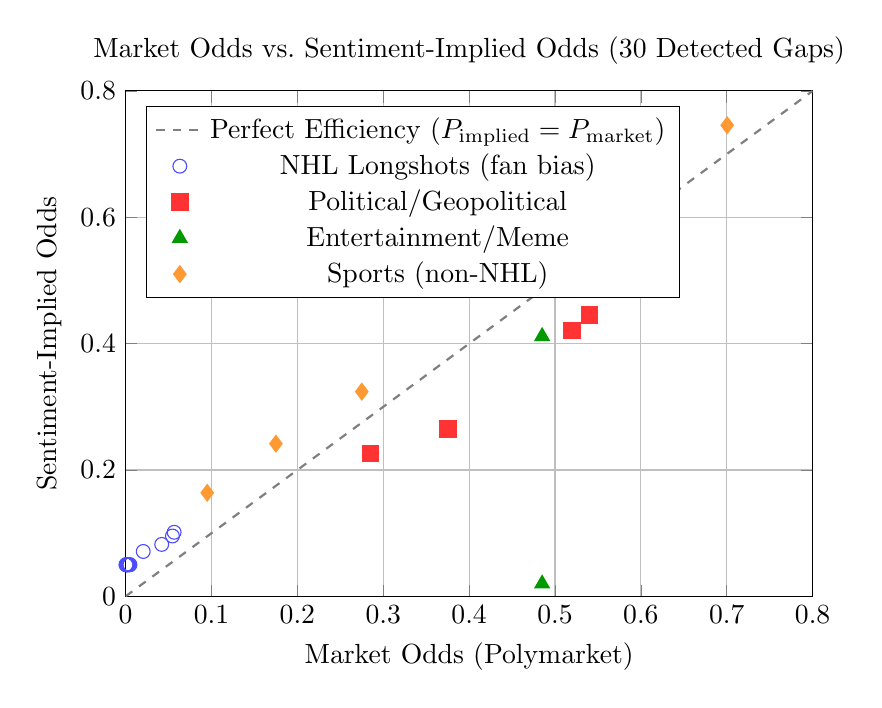
\begin{tikzpicture}
\begin{axis}[
    width=0.85\textwidth,
    height=8cm,
    xlabel={Market Odds (Polymarket)},
    ylabel={Sentiment-Implied Odds},
    xmin=0, xmax=0.8,
    ymin=0, ymax=0.8,
    grid=major,
    legend pos=north west,
    title={Market Odds vs.\ Sentiment-Implied Odds (30 Detected Gaps)}
]
% Perfect efficiency line
\addplot[domain=0:0.8, dashed, thick, gray] {x};
\addlegendentry{Perfect Efficiency ($P_{\text{implied}} = P_{\text{market}}$)}

% NHL longshots (fan bias cluster)
\addplot[only marks, mark=o, mark size=2.5, blue!70] coordinates {
    (0.0005, 0.05) (0.0005, 0.05) (0.0015, 0.05) (0.0015, 0.05)
    (0.0015, 0.05) (0.0015, 0.05) (0.0025, 0.05) (0.0035, 0.05)
    (0.0045, 0.0501) (0.005, 0.05) (0.0205, 0.071) (0.042, 0.0822)
    (0.0545, 0.0955) (0.003, 0.05) (0.0565, 0.1014)
};
\addlegendentry{NHL Longshots (fan bias)}

% Political/geo
\addplot[only marks, mark=square*, mark size=3, red!80] coordinates {
    (0.52, 0.4206) (0.375, 0.2648) (0.54, 0.4457)
    (0.615, 0.5103) (0.285, 0.2262)
};
\addlegendentry{Political/Geopolitical}

% Entertainment/meme
\addplot[only marks, mark=triangle*, mark size=3, green!60!black] coordinates {
    (0.485, 0.02) (0.485, 0.4116) (0.595, 0.6885) (0.565, 0.6247)
};
\addlegendentry{Entertainment/Meme}

% Other sports
\addplot[only marks, mark=diamond*, mark size=3, orange!80] coordinates {
    (0.095, 0.1639) (0.175, 0.2416) (0.275, 0.324) (0.7005, 0.7457)
};
\addlegendentry{Sports (non-NHL)}

\end{axis}
\end{tikzpicture}
\caption{Scatter plot of market odds vs.\ sentiment-implied odds for all 30 detected gaps. Points above the diagonal indicate bullish sentiment bias; the NHL cluster at near-zero market odds with 5\% implied odds represents systematic fan optimism, not market inefficiency.}
\label{fig:scatter}
\end{figure}

The most striking feature of Figure~\ref{fig:scatter} is the cluster of 15 NHL Stanley Cup contracts in the bottom-left corner: market odds of 0.05\%--5.6\% versus sentiment-implied odds uniformly near 5\%. This pattern is consistent with \textbf{social media selection bias}---fans of a team are disproportionately likely to post positive content about their team's championship prospects, creating a systematically bullish sentiment signal that does not reflect informed probability assessment.

This finding aligns with Xiong's (2013) work on speculative sentiment: social media selects for enthusiasm, producing a structural positive skew in sentiment data that is \textit{not} a tradable signal but rather a known property of the data-generating process.

\subsection{The Highest-Confidence Gap: A Case Study in False Positives}

The system's highest-confidence detection (98\%, 46.5\% edge) was a cross-market arbitrage on the contract ``Will Jesus Christ return before GTA VI?''---a meme market where Polymarket priced the event at 48.5\% while a competitor platform priced it at 2\%. This ``arbitrage'' reflects fundamentally different user bases pricing a joke differently, not a genuine cross-market inefficiency. The contract's low liquidity means any attempt to trade the spread would move the price more than the edge itself.

\subsection{Validation: Zero Resolved Predictions}

\begin{tcolorbox}[colback=red!5, colframe=red!60, title=Critical Finding]
After four complete analytical cycles, \textbf{zero of the 30 detected gaps have been validated} against actual market resolution. The \texttt{backtest\_results} table contains exactly zero rows. No gap has a recorded \texttt{was\_correct} value, \texttt{realized\_edge}, or \texttt{resolution\_outcome}. Without validation data, all confidence scores and edge estimates are \textbf{unverified hypotheses}.
\end{tcolorbox}

This represents the fundamental limitation of the current system: it generates predictions without tracking resolution, making it impossible to compute Brier scores, calibration curves, or any standard measure of forecast quality.

% ══════════════════════════════════════════════════════════
\section{Why the System Cannot Find Genuine Gaps}
\label{sec:why}
% ══════════════════════════════════════════════════════════

Our analysis identifies five structural reasons why daily-frequency sentiment-based gap detection fails against Polymarket:

\subsection{Speed Mismatch (The Kyle Problem)}

In Kyle's (1985) framework, the information half-life $\tau_{1/2}$ determines how quickly new information is incorporated into prices. For liquid Polymarket contracts:

\begin{equation}
    \tau_{1/2}^{\text{Polymarket}} \approx \text{minutes to hours}
\end{equation}

Our system operates at:

\begin{equation}
    \tau_{\text{cycle}} \approx 6{,}917\text{s} \approx 1.9\text{ hours (per cycle)} \quad \text{with 1 cycle/day}
\end{equation}

The effective detection latency---from information emergence to gap flagging---is \textbf{12--24 hours}, far exceeding $\tau_{1/2}$. Any genuine gap has been closed by informed traders long before our system detects it.

\subsection{No Information Advantage}

The system reads the same public sources (Reddit, Bluesky, news RSS) that Polymarket participants read. It has no proprietary data, no insider information, and no access to non-public signals. Its only potential advantage is \textit{processing speed}---running NLP on sources faster than human reading---but this advantage is negated by the daily cycle frequency.

\subsection{Sentiment $\neq$ Information}

Equation~\ref{eq:implied_prob} assumes that aggregate sentiment maps linearly to probability via parameter $\alpha$. This assumption fails for several reasons:

\begin{itemize}
    \item Social media sentiment is \textbf{structurally biased positive} (fans, enthusiasts, and advocates post more than critics)
    \item Sentiment intensity does not correlate with information quality (a passionate fan post and an expert analysis receive equal weight)
    \item The mapping parameter $\alpha = 0.4$ is \textbf{not calibrated}---it was set heuristically, not derived from historical data
\end{itemize}

\subsection{Insufficient Historical Data}

With only 8 records in the \texttt{historical\_odds} table, the pattern deviation detector (Type 3) and information asymmetry detector (Type 2) have inadequate data for statistical analysis. The z-score computation requires sufficient samples to estimate $\mu$ and $\sigma$ reliably; with $n = 8$, confidence intervals are too wide for meaningful anomaly detection.

\subsection{Liquidity Constraint}

Even if a genuine gap were detected in an illiquid market, the cost of executing the trade (bid-ask spread + market impact) would likely exceed the edge. For the NHL longshot contracts where most gaps were detected, a single large order would move the price substantially, eliminating the edge before it could be captured.

% ══════════════════════════════════════════════════════════
\section{What Would Be Required}
\label{sec:required}
% ══════════════════════════════════════════════════════════

Based on our analysis, a system capable of detecting genuine prediction market inefficiencies would require:

\begin{table}[H]
\centering
\caption{Gap analysis: current system vs.\ requirements for viable gap detection.}
\label{tab:gap_analysis}
\begin{tabular}{@{}p{3.5cm}p{4.5cm}p{4.5cm}@{}}
\toprule
\textbf{Dimension} & \textbf{Current System} & \textbf{Required System} \\
\midrule
Cycle Frequency & 1$\times$/day (8 PM) & Every 5--15 minutes \\
Information Sources & Public social media & Event-driven feeds, filings, insider-adjacent data \\
Sentiment Calibration & Uncalibrated ($\alpha = 0.4$) & Source-specific calibration curves \\
Market Universe & 625 contracts (broad) & 10--20 liquid, catalyst-rich contracts \\
Validation & 0 resolved predictions & 30+ days of tracked resolutions \\
Backtesting & Framework exists, 0 data & 3--6 months historical backtest \\
Historical Odds & 8 records & Continuous tick-level price history \\
Execution & Analysis only & Integrated order placement \\
\bottomrule
\end{tabular}
\end{table}

% ══════════════════════════════════════════════════════════
\section{Alternative Application: Prediction Market Odds as Equity Signal Features}
\label{sec:future}
% ══════════════════════════════════════════════════════════

While our system fails to generate tradable signals \textit{within} prediction markets, the infrastructure has a potentially valuable alternative application: using Polymarket odds as \textbf{input features for equity forecasting models}.

\subsection{Theoretical Basis}

Prediction market prices on policy events (Federal Reserve rate decisions, tariff announcements, geopolitical conflicts) encode the market's consensus probability of outcomes that directly affect equity valuations. These probabilities are:

\begin{itemize}
    \item \textbf{Forward-looking:} Unlike economic indicators (lagging) or surveys (slow-updating), prediction market prices update in real-time as new information arrives.
    \item \textbf{Incentive-aligned:} Participants have financial stakes in accuracy, unlike survey respondents.
    \item \textbf{Continuously available:} Unlike quarterly earnings or monthly employment reports, prediction market odds are available 24/7.
\end{itemize}

\subsection{Proposed Integration}

Polymarket odds on macro-relevant events could serve as features in time-series forecasting models such as Temporal Fusion Transformers (TFT) \citep{lim2021temporal}. TFT models are particularly well-suited because they:

\begin{enumerate}
    \item Handle mixed-frequency inputs (daily equity prices + real-time prediction market odds)
    \item Provide interpretable attention weights showing \textit{which} prediction market features drive equity forecasts
    \item Support static (contract metadata), known future (event dates), and observed (odds history) input types natively
\end{enumerate}

Example features: Fed rate cut probability, tariff escalation probability, ceasefire probability, election outcome odds---each representing a macro risk factor that traditional factor models cannot easily capture.

\subsection{Why This May Succeed Where Direct Trading Failed}

The key distinction is that equity markets are \textit{not} directly pricing prediction market odds. While Polymarket participants rapidly incorporate information into prediction market prices, the \textit{equity implications} of those probabilities may be underappreciated by stock market participants. This creates a potential information asymmetry that our data pipeline is well-positioned to exploit---not by trading prediction markets, but by using their odds as a novel feature class for equity models.

% ══════════════════════════════════════════════════════════
\section{Conclusion}
% ══════════════════════════════════════════════════════════

This paper presents a comprehensive multi-agent system for prediction market pricing gap detection, demonstrating both the engineering feasibility of large-scale sentiment-driven market analysis and the economic reality of attempting to outperform informationally efficient markets with public data at low frequency.

Our key findings are:

\begin{enumerate}
    \item \textbf{The architecture works; the signal does not.} The system successfully collects, processes, and analyzes 32,791 social posts across 625 contracts using ensemble NLP, but the detected ``gaps'' reflect social media optimism bias rather than genuine market inefficiency.

    \item \textbf{Polymarket is consistent with weak-form efficiency for liquid contracts.} The market incorporates public information faster than a daily-frequency analytical system can detect divergences.

    \item \textbf{The speed gap is structural, not fixable by optimization.} Even reducing cycle time from 2 hours to 5 minutes would not close the gap with informed traders who monitor these markets continuously.

    \item \textbf{Prediction market odds as equity features represent a more promising application.} The infrastructure built for this project---multi-source data collection, sentiment analysis, database persistence---can be repurposed to generate novel features for equity forecasting models.
\end{enumerate}

The negative result itself is informative: it provides empirical evidence for prediction market efficiency from the perspective of an automated system attempting to exploit inefficiencies, complementing the theoretical literature with a practical engineering perspective.

% ══════════════════════════════════════════════════════════
% REFERENCES
% ══════════════════════════════════════════════════════════

\begin{thebibliography}{20}

\bibitem[Arrow et al., 2008]{arrow2008promise}
Arrow, K.~J., Forsythe, R., Gorham, M., et al. (2008).
\newblock The promise of prediction markets.
\newblock \textit{Science}, 320(5878):877--878.

\bibitem[Bollen et al., 2011]{bollen2011twitter}
Bollen, J., Mao, H., \& Zeng, X. (2011).
\newblock Twitter mood predicts the stock market.
\newblock \textit{Journal of Computational Science}, 2(1):1--8.

\bibitem[Hutto \& Gilbert, 2014]{hutto2014vader}
Hutto, C. \& Gilbert, E. (2014).
\newblock {VADER}: A parsimonious rule-based model for sentiment analysis of social media text.
\newblock \textit{Proceedings of the International AAAI Conference on Web and Social Media}, 8(1).

\bibitem[Kyle, 1985]{kyle1985continuous}
Kyle, A.~S. (1985).
\newblock Continuous auctions and insider trading.
\newblock \textit{Econometrica}, 53(6):1315--1335.

\bibitem[Lim et al., 2021]{lim2021temporal}
Lim, B., Ar{\i}k, S.~{\"O}., Loeff, N., \& Pfister, T. (2021).
\newblock Temporal fusion transformers for interpretable multi-horizon time series forecasting.
\newblock \textit{International Journal of Forecasting}, 37(4):1748--1764.

\bibitem[Manski, 2006]{manski2006interpreting}
Manski, C.~F. (2006).
\newblock Interpreting the predictions of prediction markets.
\newblock \textit{Economics Letters}, 91(3):425--429.

\bibitem[Wolfers \& Zitzewitz, 2004]{wolfers2004prediction}
Wolfers, J. \& Zitzewitz, E. (2004).
\newblock Prediction markets.
\newblock \textit{Journal of Economic Perspectives}, 18(2):107--126.

\end{thebibliography}

\end{document}
